\chapter{Розробка рішень для ІС за видами забезпечення} 
\label{chap:third}

\section{Інформаційне забезпечення}

Для роботи ІС з користувачами - підтримки функціоналу зберігання і відтворення моделей система використовує SQL БД:

Структура БД наведена нижче:

\begin{center}

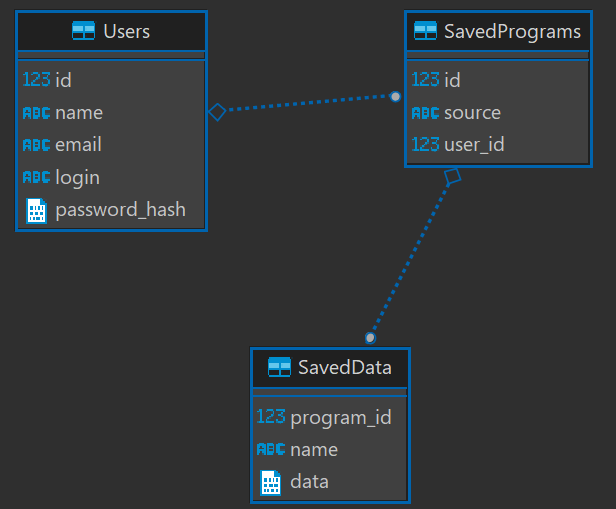
\includegraphics[width=12cm]{db_er_diagram}

Рисунок 3.1 - Схема таблиць бази даних
\end{center}

ІС для корректного функіонування та збереження можливості подальших змін повинна бути поділена на модулі.

Перелік, взаємозв'язки та призначення модулів наведено нижче:

\begin{center}

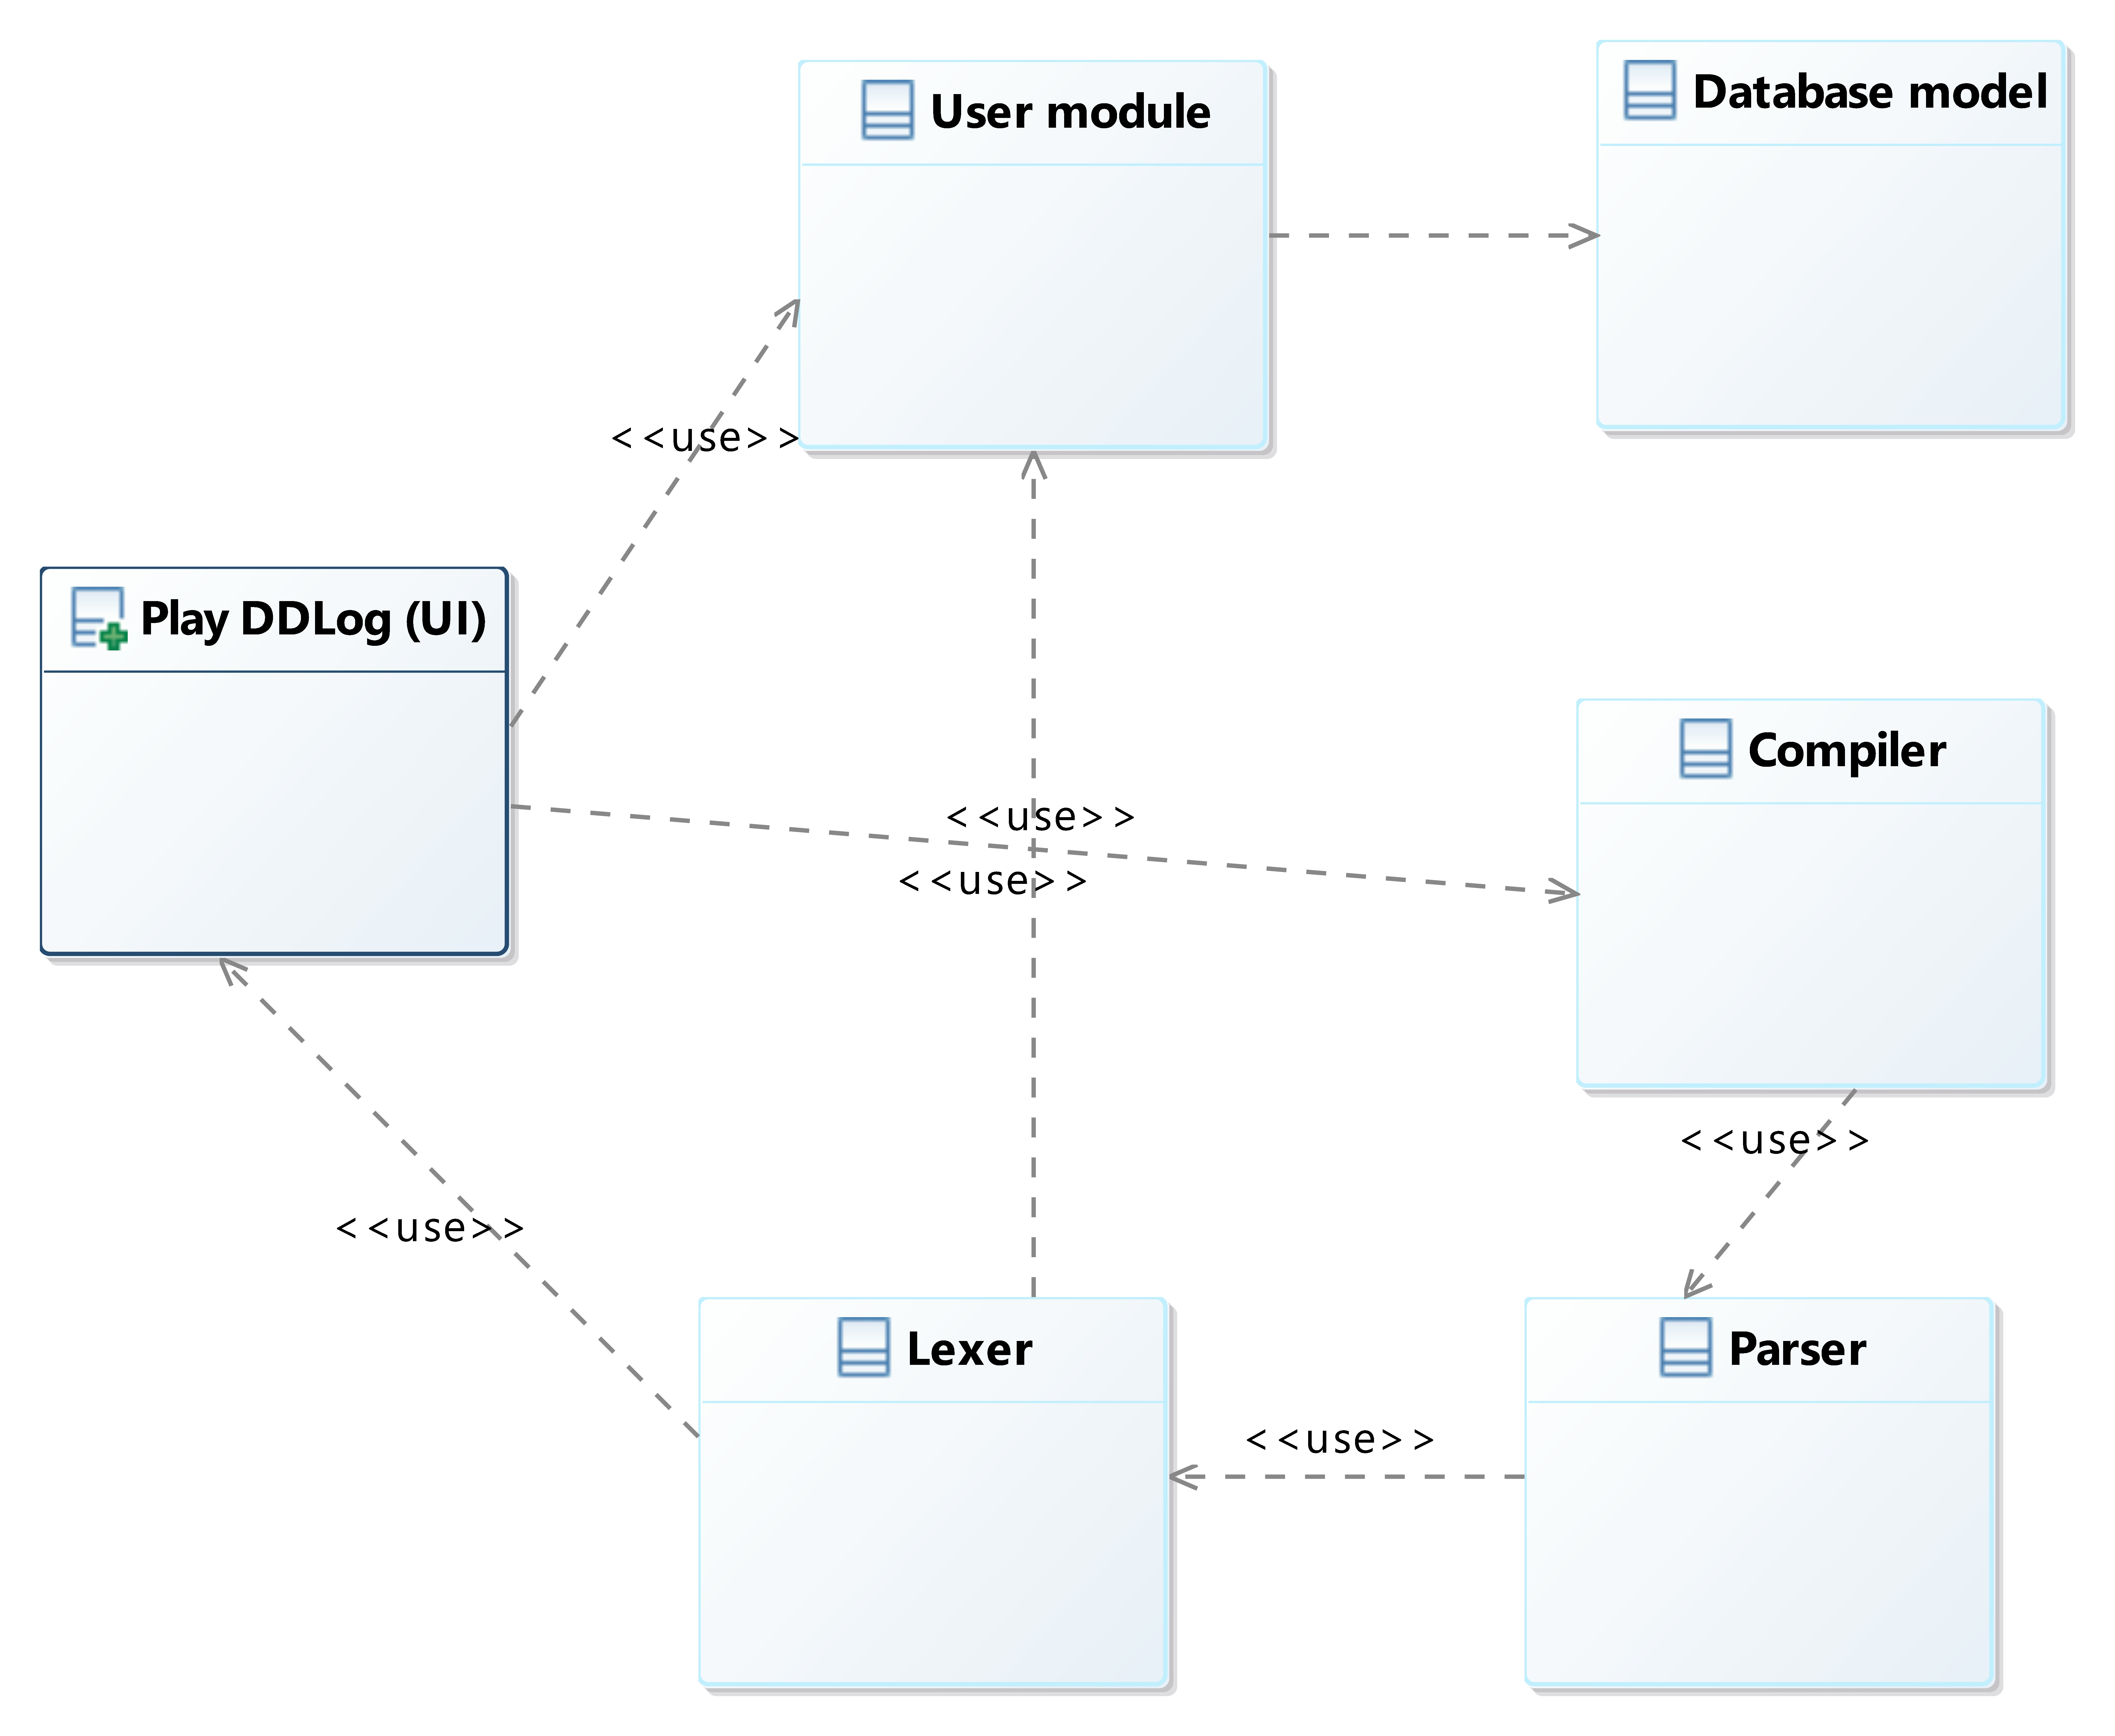
\includegraphics[width=12cm]{class_diagram}

Рисунок 3.2 - Діаграма класів (для бізнес логіки)
\end{center}

Для взаємодією браузерної частини ІС з серверною обрано архітектурний підхід REST а за форматом кодування обрано JSON.

Конкретні типи повідомленнь майже неможливо розробити наперед, а тому вони повинні бути визначені на етапі розробки, тут їх визначено не буде.

\section{Організаційне забезпечення}

При взаємодії з системою можна виділити ключові точки, що зображені на діаграммі станів нижче.

\begin{center}

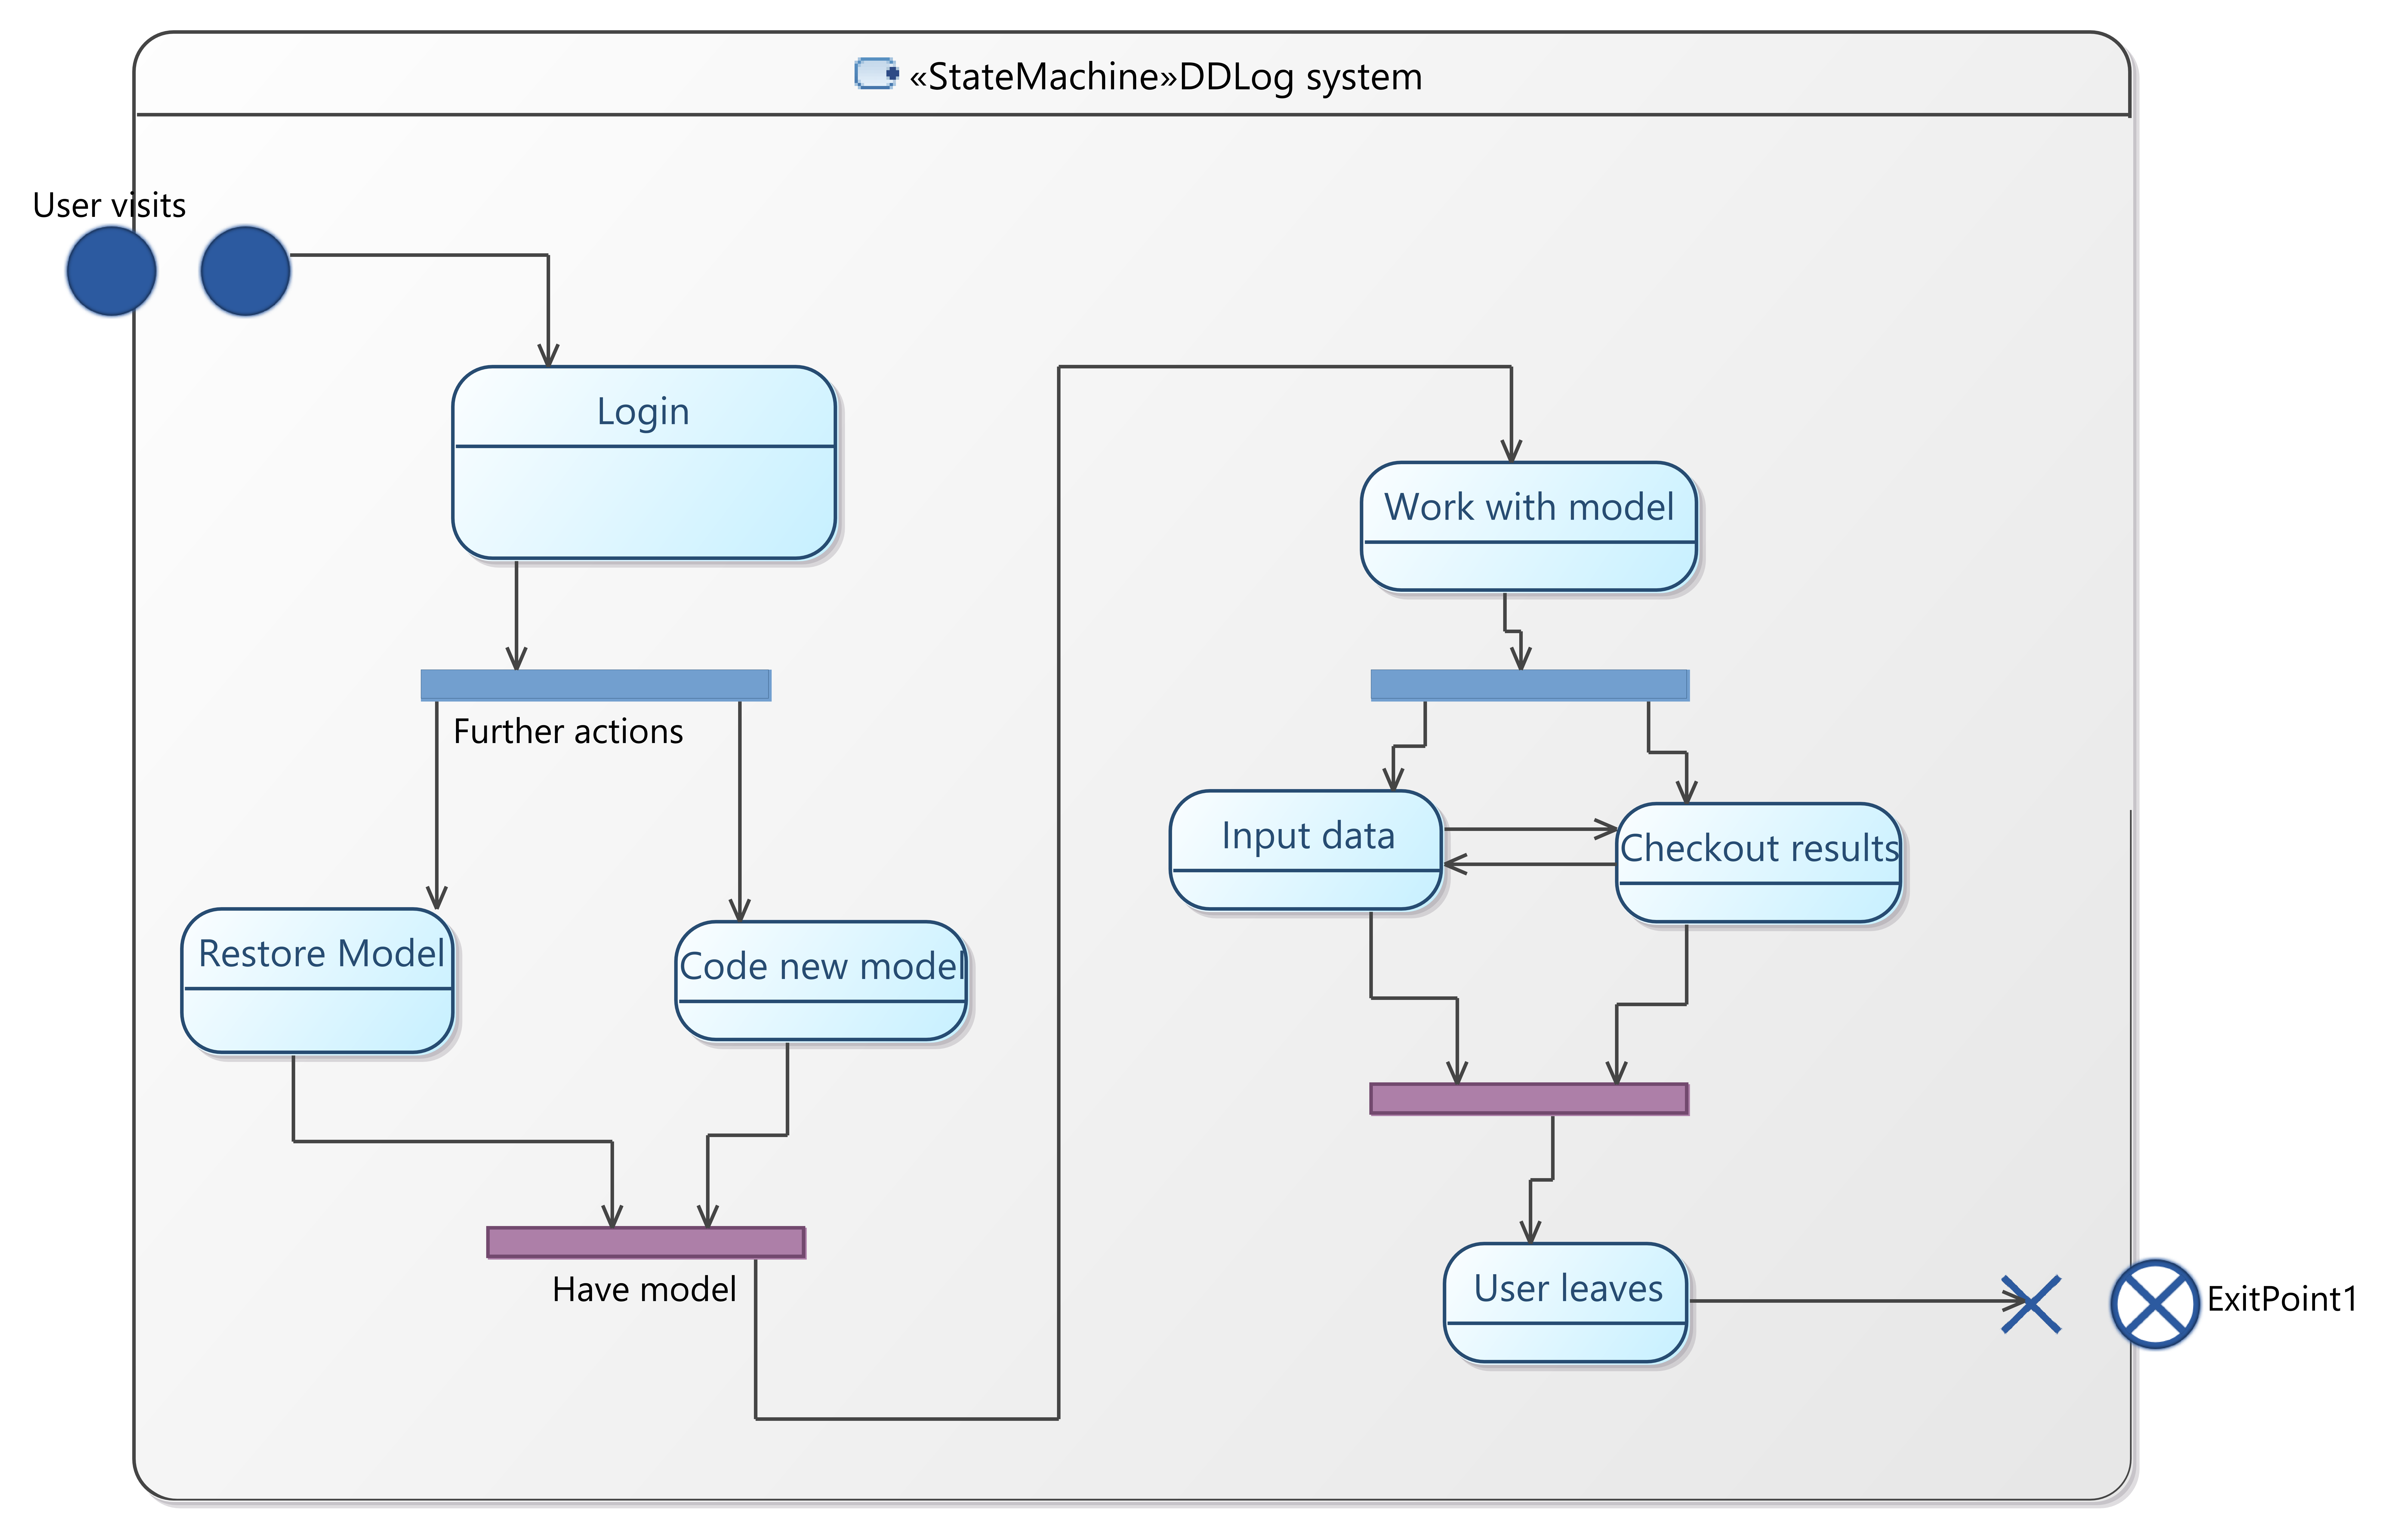
\includegraphics[width=12cm]{user_state_machine}

Рисунок 3.3 - Діаграмма станів користувача
\end{center}

Користувач 

\section{Програмне забезпечення}

При проектуванні програмного забезпечення мають бути вироблені рішення щодо системного і прикладного програмного забезпечення.
Для ілюстрації структури прикладного програмного забезпечення наводяться діаграми компонентів (UML).

Окрім внутрішньої організації модулів для змістовної частини ІС існує ще невідємна потреба в інфраструктурних модулях ІС. Наприклад -  робота з веб протоколами.

Загальну структуру компонентів ІС наведено нижче:

\begin{center}

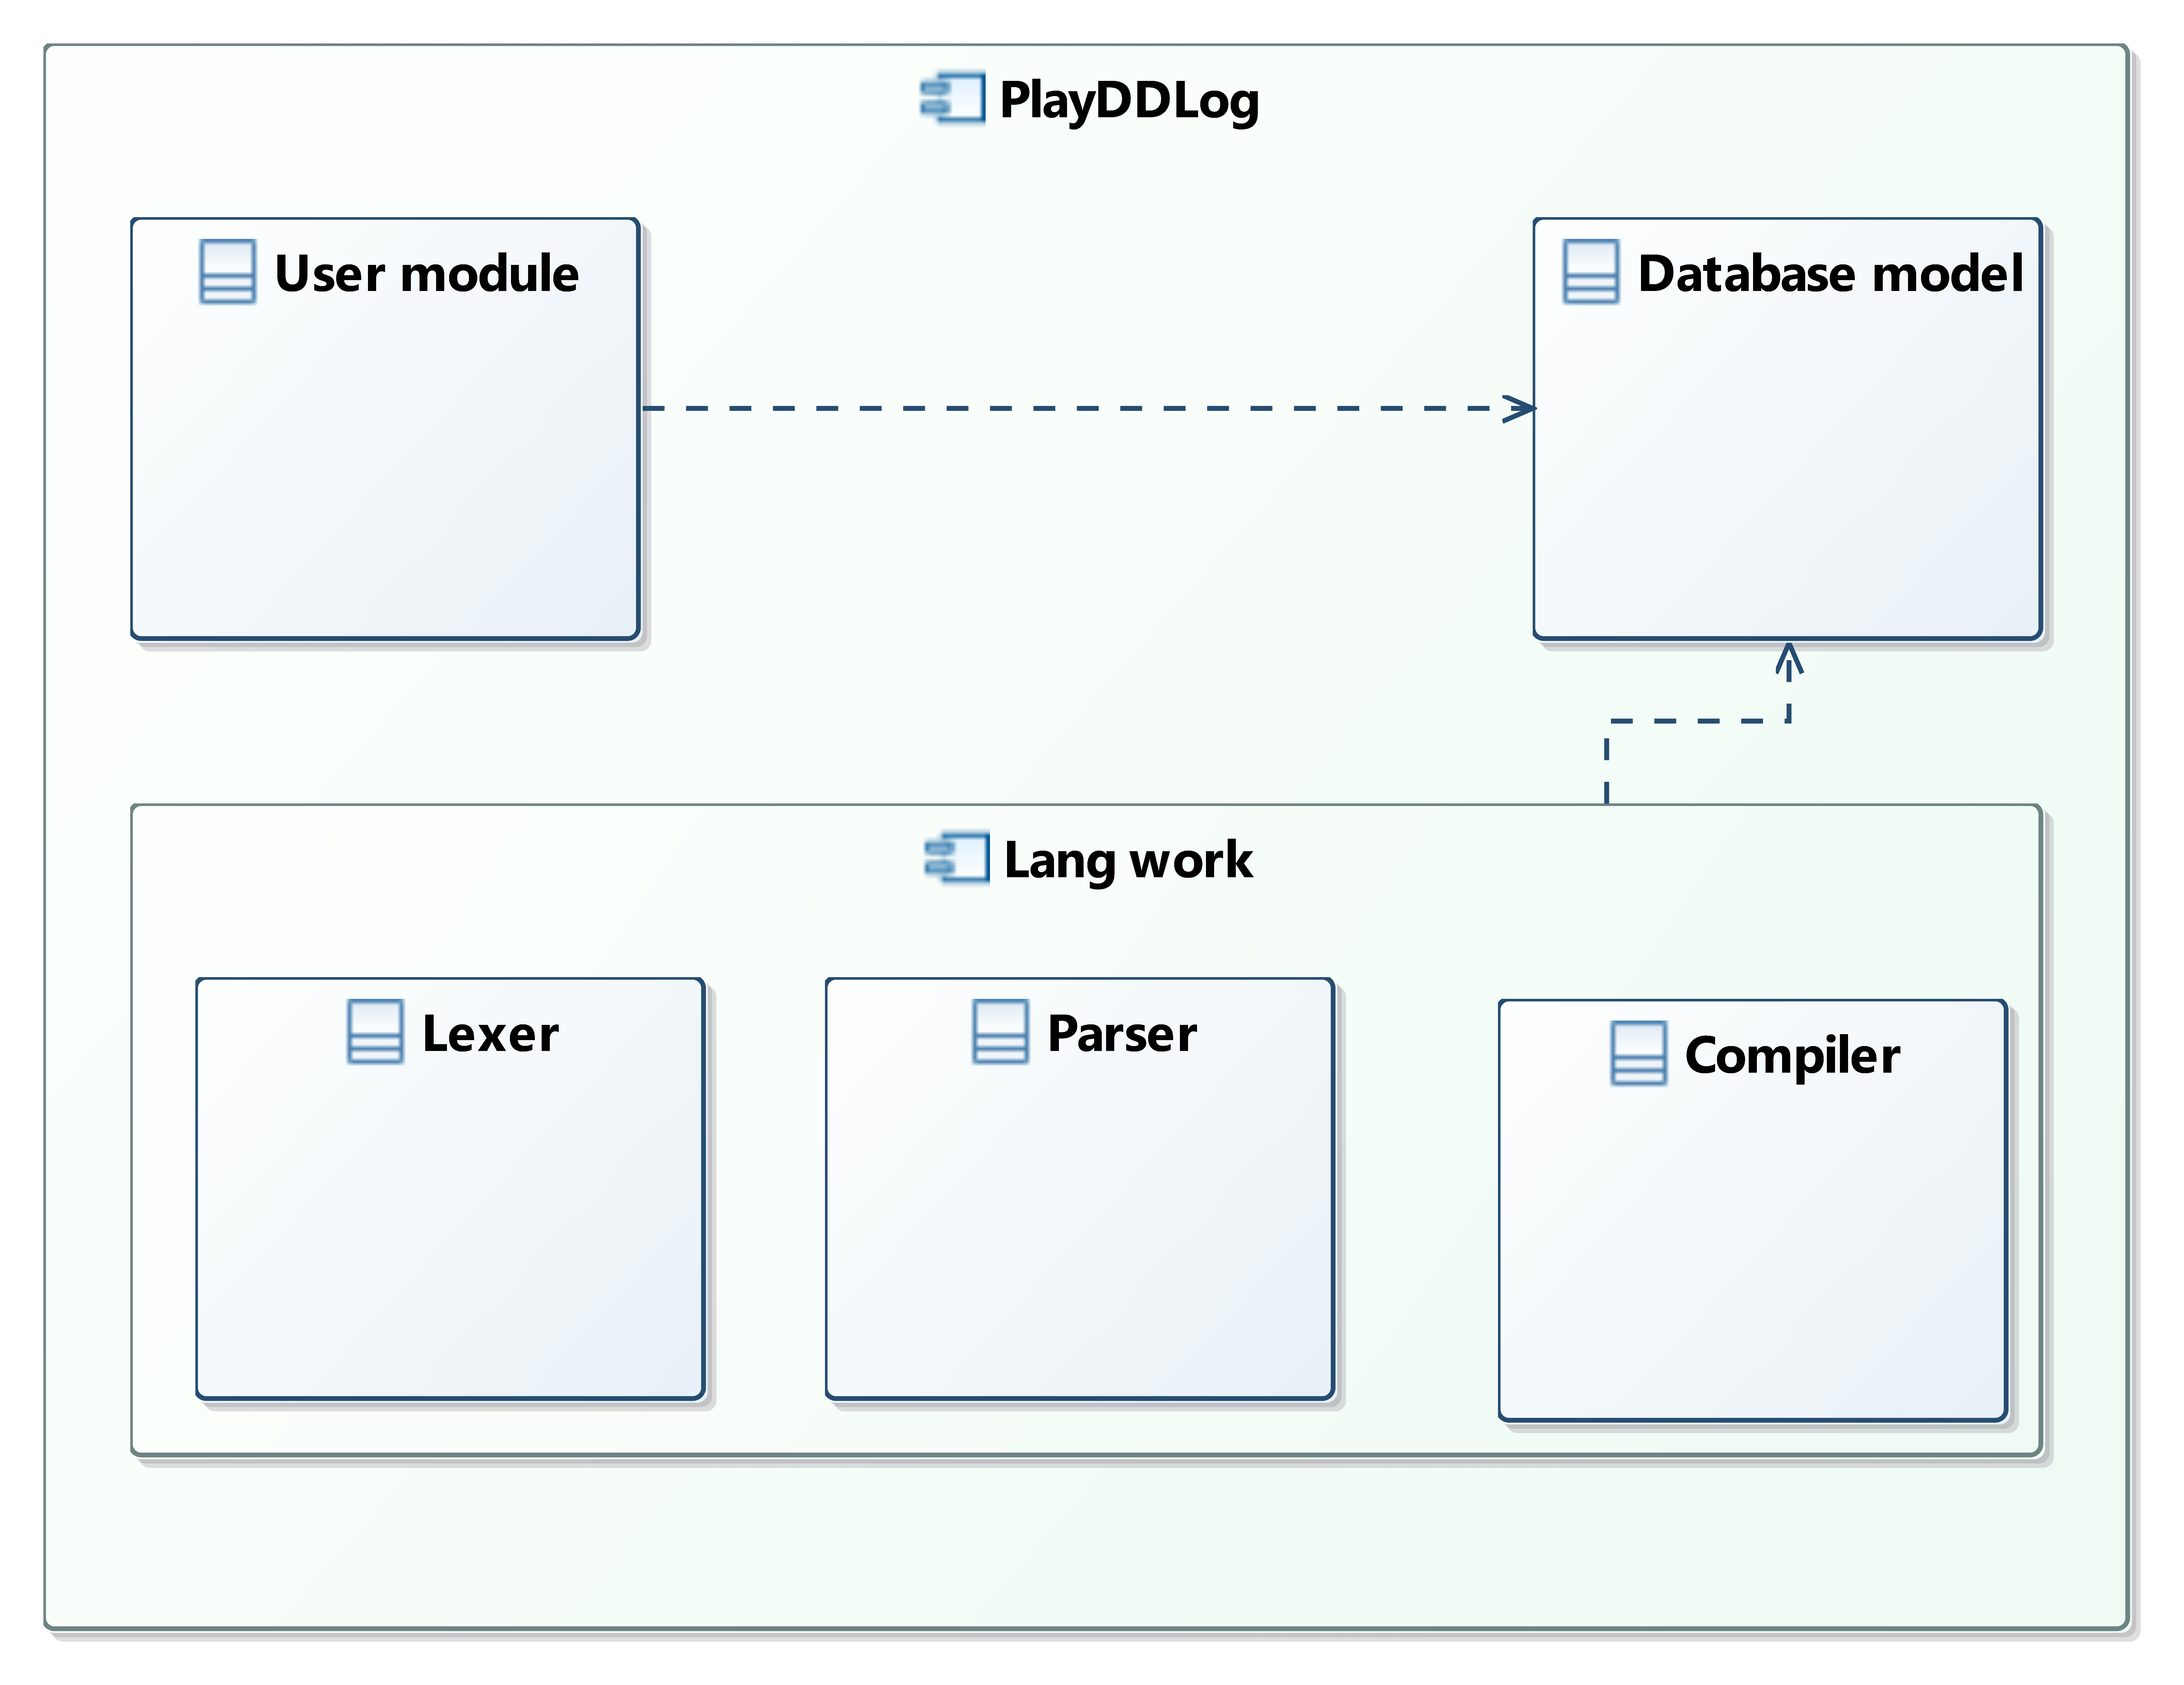
\includegraphics[width=12cm]{component_diagram}

Рисунок 3.4 - Діаграмма компонентів
\end{center}

Конкретний код ІС та цього документу знаходиться в git-репозиторії за посиланням: \cite{repo}

\section{Технічне забезпечення}

Комплекс технічних засобів обрано як для розгортання веб додатку. Це включає в себе:

\begin{enumerate}

\item Сервер що обслуговує запити на веб сторінки;

\item Сервер що обслуговує запити до API;

\item СКБД для роботи з БД.

\end{enumerate}

Кінцевий вигляд розгорнутої системи наведено нижче:

\begin{center}


\includegraphics[width=12cm]{deploy_diagram}

Рисунок 3.5 - Діаграмма розгортання

\end{center}

Взагалі, всі компоненти ІС можуть виконуватися як на одній, так і на різних комп'ютерах.  Вони можуть бути як фізичні, так і віртуальні (ВМ). Весь комплекс ПЗ може виконуватись як в рамках однієї ВМ, так і на великому комплексі серверів.

